\documentclass{standalone}
\usepackage{amsmath,amssymb}
\usepackage[dvipsnames]{xcolor}
\usepackage{tikz} 
\usetikzlibrary{arrows, decorations.markings,decorations.pathreplacing,angles,quotes}
\usepackage{microtype}
\usepackage{fourier}

\definecolor{np}{rgb}{0.5, 0, 0.5}
\definecolor{no}{rgb}{1,0.65,0}
\definecolor{nb}{rgb}{0,0,1}
\definecolor{ng}{rgb}{0,0.5,0}

%include other needed packages here   
\begin{document}

\begin{tikzpicture}
% include your tikz code here
    		\node[anchor=south west,inner sep=0] (Bild) at (0,0) {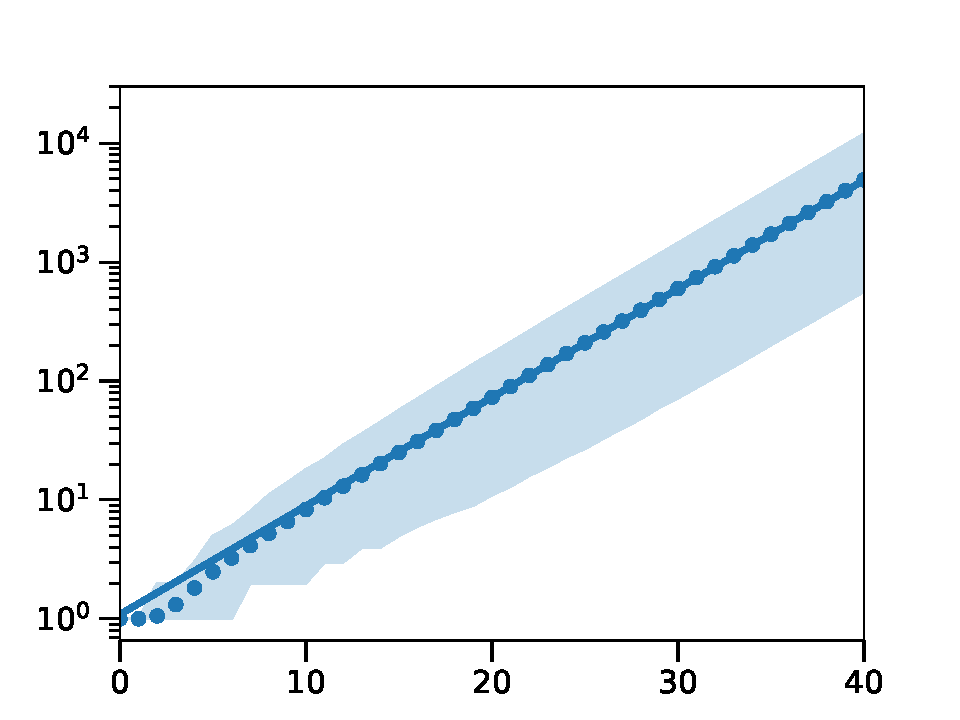
\includegraphics[scale=0.39]{fig2a_blank.pdf}};
   		\begin{scope}[x=(Bild.south east),y=(Bild.north west)]
        	\draw (0.55,-0.035) node {time $t$ [days]};
        	\draw (-0.01,0.5) node [rotate=90] {epidemic size $I_{\text{surv}}(t)$};
    		\end{scope}
\end{tikzpicture}

\end{document}